\section{Realisierung}
\label{sec:Realisierung}

TODO: Libraries, Umgebung, Architektur

\subsection{Architektur}
\begin{figure}
    \centering
    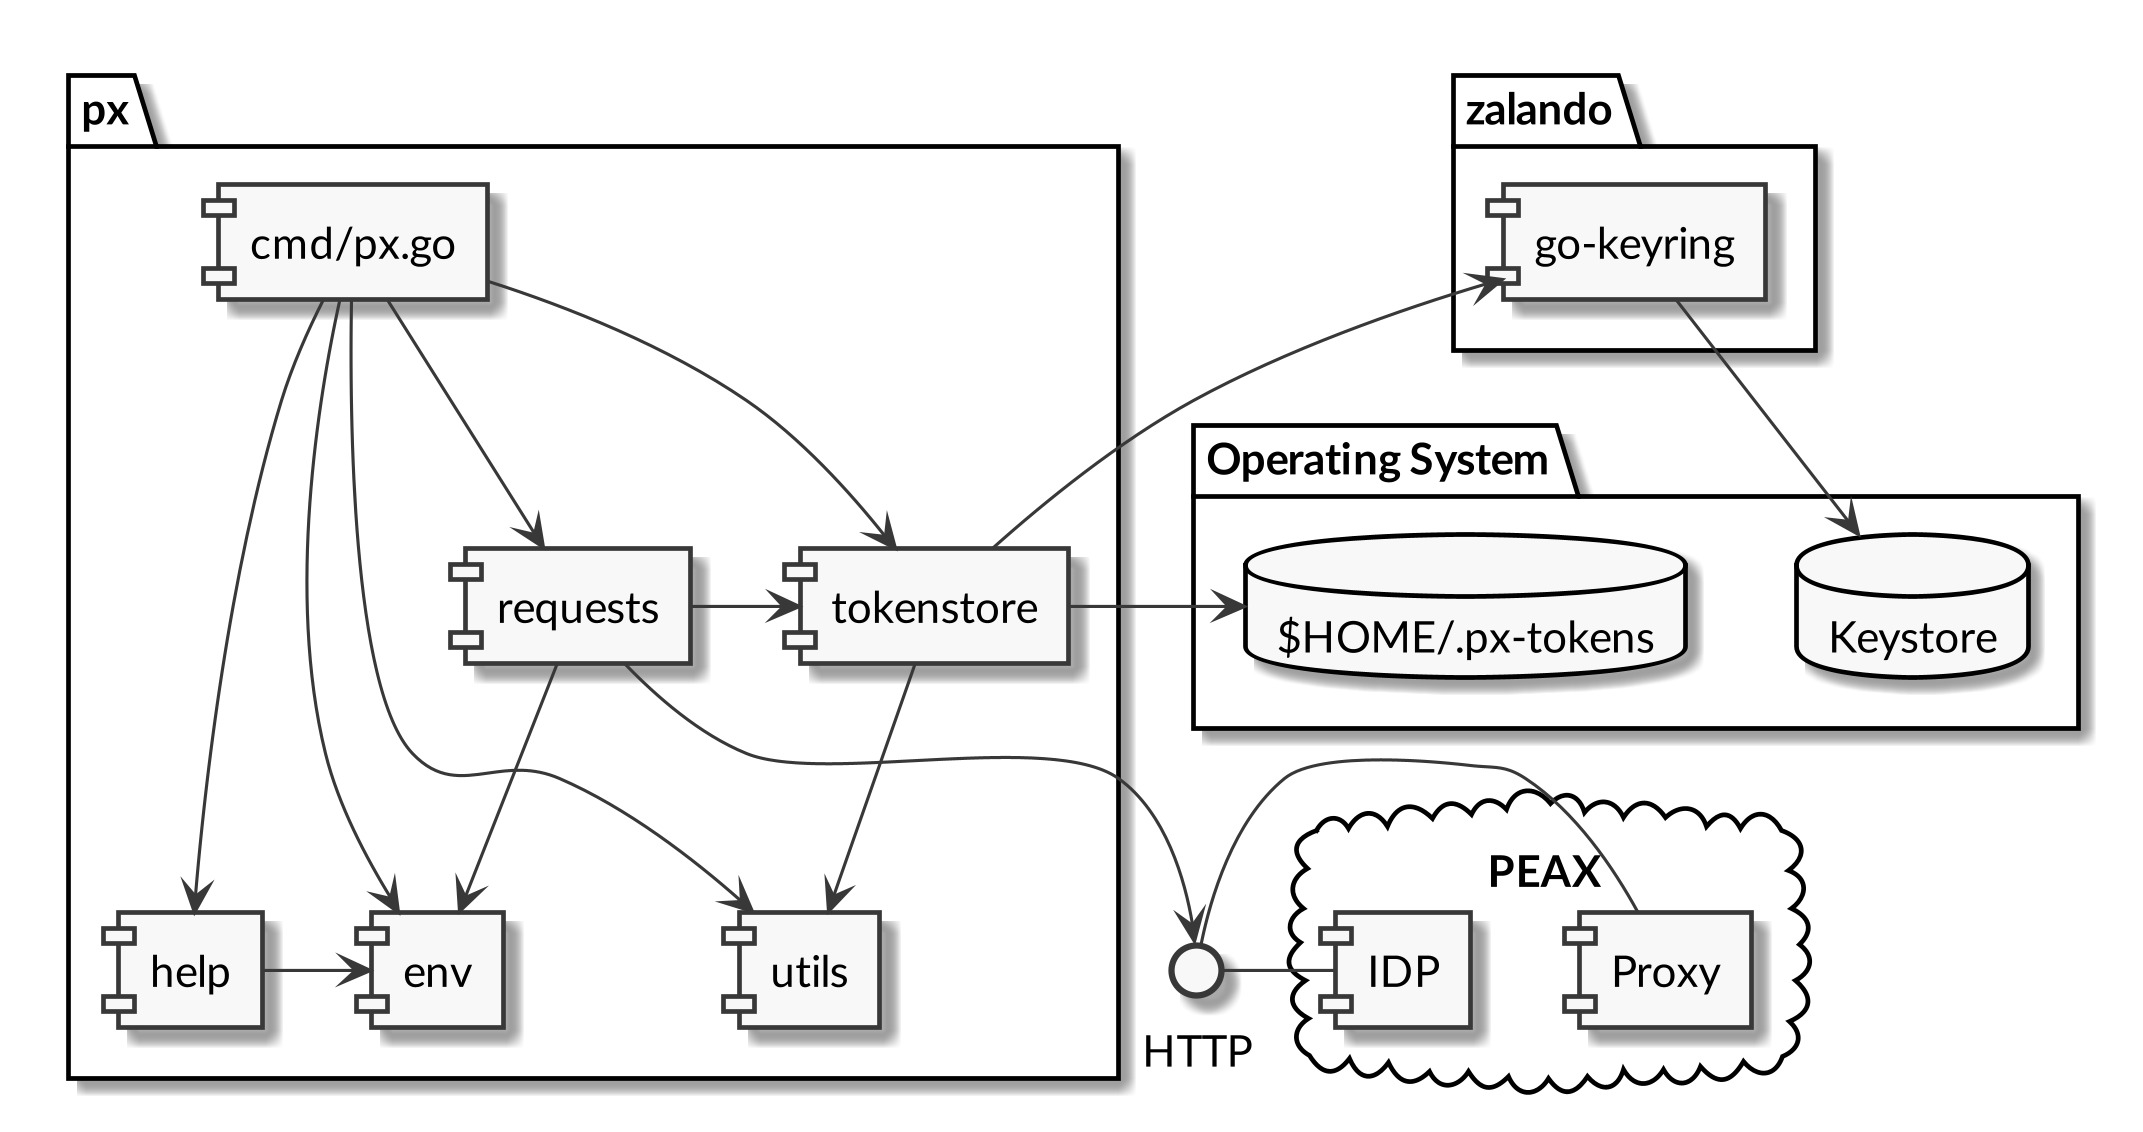
\includegraphics[width=\linewidth]{pics/komponentendiagramm.png}
    \caption{Komponentendiagramm: Die Komponentenarchitektur von \texttt{px}}
\end{figure}

\subsection{Zwei-Faktor-Authentifizierung}

\begin{figure}
    \centering
    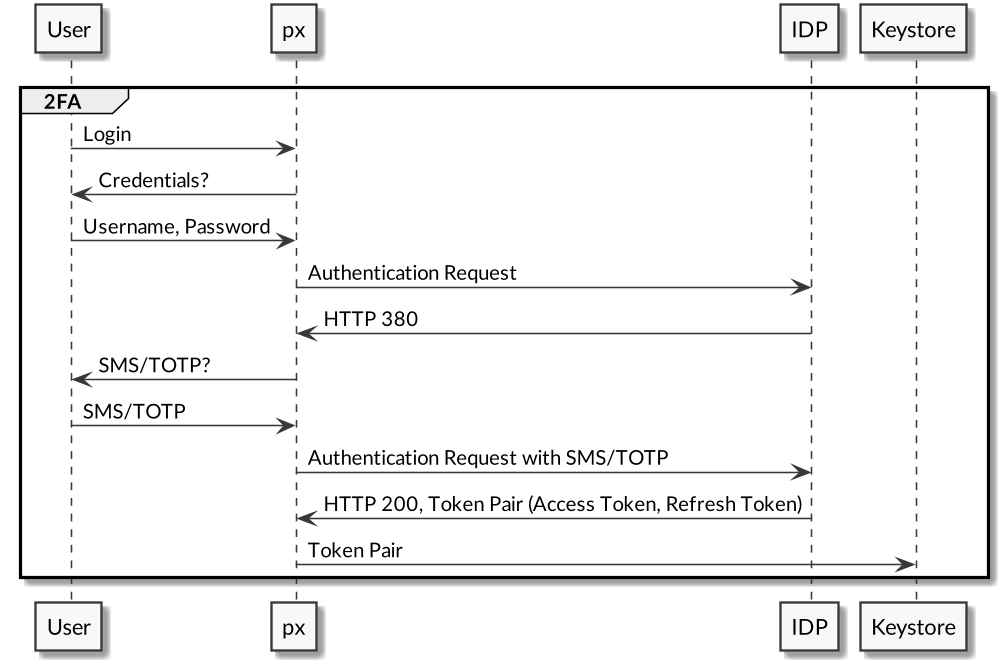
\includegraphics[width=\linewidth]{pics/sequence-2fa.png}
    \caption{Sequenzdiagramm: Der Ablauf der Zwei-Faktor-Authentifizierung}
\end{figure}

\subsection{Retry-Mechanismus}

\begin{figure}
    \centering
    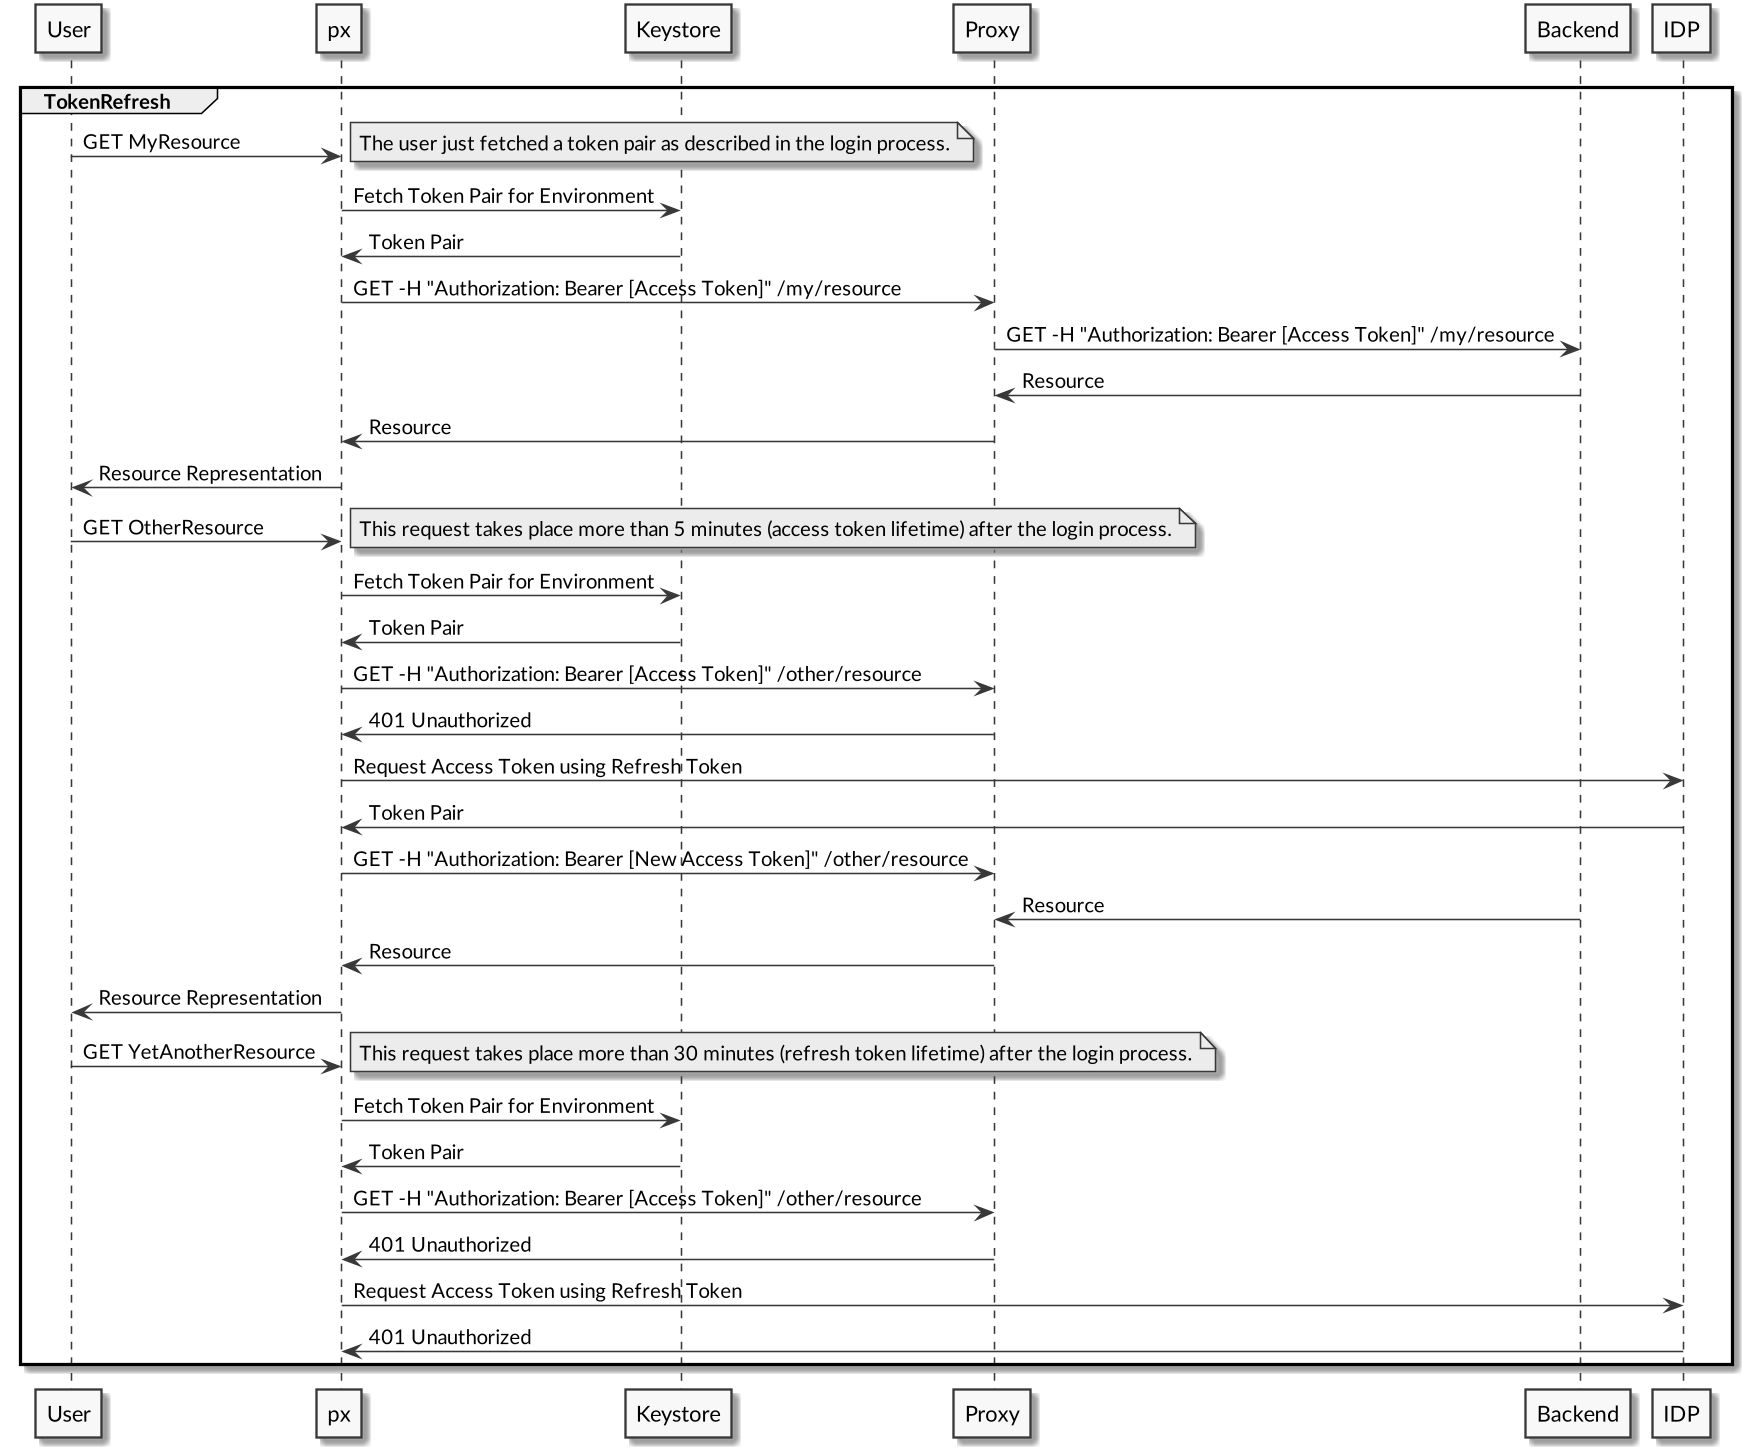
\includegraphics[width=\linewidth]{pics/sequence-retry.png}
    \caption{Sequenzdiagramm: Der für den Benutzer transparente Retry-Mechanismus mit aktualisiertem Access Token}
\end{figure}

\subsection{Token-Store}

TODO: sicher und unsicher, Datenstruktur
